

% Diagram of Android activity life cycle
% Author: Pavel Seda 
\documentclass[border=10pt]{standalone}
\usepackage{tikz}
\usetikzlibrary{arrows.meta}
\tikzset{%
	>={Latex[width=2mm,length=2mm]},
	% Specifications for style of nodes:
	base/.style = {rectangle, rounded corners, draw=black,
		minimum width=4cm, minimum height=1cm,
		text centered, font=\sffamily},
	activityStarts/.style = {base, fill=blue!30},
	startstop/.style = {base, fill=red!30},
	activityRuns/.style = {base, fill=green!30},
	processmini/.style = {base, draw=pink!90, minimum width=0.5cm, fill=orange!15,
		font=\ttfamily},
	process/.style = {base, draw=pink!90, minimum width=2.5cm, fill=orange!15,
		font=\ttfamily},
}
\begin{document}    
	% Drawing part, node distance is 1.5 cm and every node
	% is prefilled with white background
	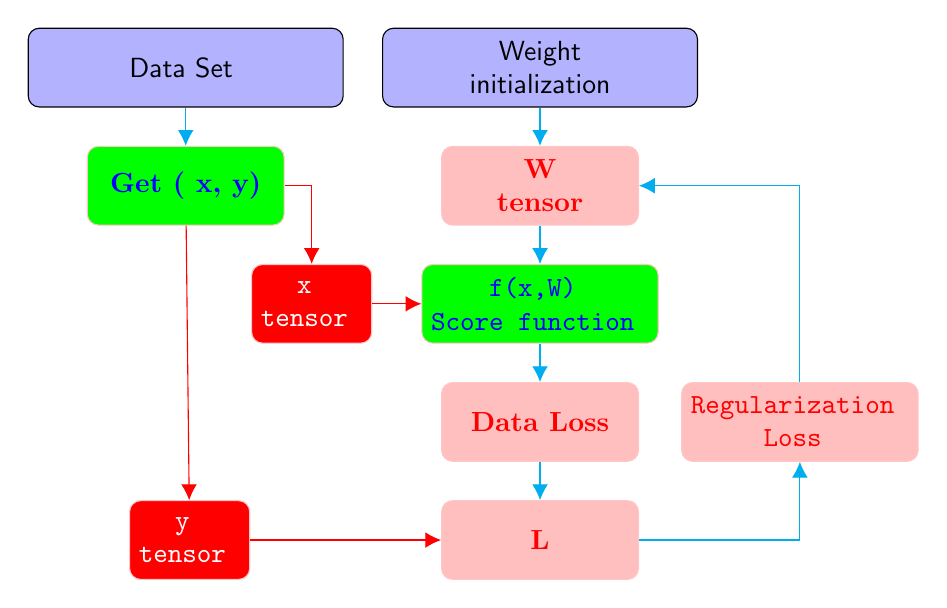
\begin{tikzpicture}[node distance=1.5cm,
		every node/.style={fill=white, font=\sffamily}, align=center]
		
		% Specification of nodes (position, etc.)
		\node (start)             [activityStarts]              
		{  Data Set };
		
		
	
		
		
		\node (activityRuns2)      [process, below of=start , fill = green]	{\textcolor{blue}{ \bf{  Get ( x, y) }}};
		
		\node (startAD)     [ activityStarts, right of=start , xshift=3cm ]              
		{Weight \\ initialization     };
		
		\node (onCreateBlockAD)     [process, below of=startAD , fill =pink]          {\textcolor{red}{ \bf{ W }} \\ \textcolor{red}{ \bf{ tensor }}};
	
		
			
		
		\node (onCreateBlockAD1)     [process, below of=onCreateBlockAD , fill =green]      {\textcolor{blue}{  f(x,W)   } \\ \textcolor{blue}{ Score function }};
		
		
			
		\node (onCreateBlockAD6)     [processmini, left  of=onCreateBlockAD1 , fill =red, xshift=-1.4cm]          {\textcolor{white}{  x   } \\ \textcolor{white}{ tensor }};
		
		
		
		
		\node (onCreateBlockAD2)     [process, below of=onCreateBlockAD1 , fill =pink]          {\textcolor{red}{ \bf{ Data Loss }}};
		
			
		\node (onCreateBlockAD5)     [process, right of=onCreateBlockAD2 , fill =pink, xshift=1.8cm]          {\textcolor{red}{  Regularization  }  \\ \textcolor{red}{  Loss }  };
		
		
		\node (onCreateBlockAD4)     [process, below of=onCreateBlockAD2 , fill =pink]          {\textcolor{red}{ \bf{L}}};
		
			\node (ybox1)     [processmini, left of=onCreateBlockAD4 , fill =red, xshift=-2.95cm]         {\textcolor{white}{  y   } \\ \textcolor{white}{ tensor }};
			
		
		\draw[->]  [color= cyan]  (start) -- (activityRuns2);
	
		
		\draw[->]  [color= cyan]   (onCreateBlockAD4)  -| (onCreateBlockAD5);
		
		\draw[->]  [color= cyan]   (onCreateBlockAD5)  |- (onCreateBlockAD);
		
		\draw[->]  [color= cyan] (startAD)  -- (onCreateBlockAD);
		\draw[->]  [color= cyan](onCreateBlockAD)  -- (onCreateBlockAD1);
		
		\draw[->]  [color= cyan](onCreateBlockAD1)  -- (onCreateBlockAD2);
		
		\draw[->]  [color= cyan](onCreateBlockAD2)  -- (onCreateBlockAD4);
		
	
		\draw[->]  [color= red](activityRuns2)  -| (onCreateBlockAD6);
		
		\draw[->]  [color= red](onCreateBlockAD6)  -- (onCreateBlockAD1);
		
		\draw[->]  [color= red](ybox1)  -- (onCreateBlockAD4);
			
		\draw[->]  [color= red](activityRuns2)  -- (ybox1);
		
		
	\end{tikzpicture}
\end{document}